% ============================================================
% Question Bank: ch06-04 Constructing Triangles from Three Measurements
% Topic Title: Constructing Triangles from Three Measurements
% CCSS: 7.G.A.2
% Questions: 30 (18 MC + 7 SA + 5 Graphical)
% ============================================================

% --- Multiple Choice Questions (18) ---

\begin{practiceQuestion}{6-4-q01}{mc}
\begin{questionText}
A triangle has sides $6$ cm, $8$ cm, and $10$ cm. How many triangles can be constructed with these measurements?
\end{questionText}
\choiceA{None}
\choiceB{Exactly one}
\choiceC{Exactly two}
\choiceD{Infinitely many}
\correctAnswer{B}
\explanation{SSS with valid lengths produces exactly one unique triangle. Check: $6 + 8 = 14 > 10$, $6 + 10 = 16 > 8$, $8 + 10 = 18 > 6$. All pass.}
\end{practiceQuestion}

\begin{practiceQuestion}{6-4-q02}{mc}
\begin{questionText}
A triangle has angles $40°$, $60°$, and $80°$. How many different triangles can be drawn?
\end{questionText}
\choiceA{None}
\choiceB{Exactly one}
\choiceC{Exactly three}
\choiceD{Infinitely many}
\correctAnswer{D}
\explanation{AAA determines the shape but not the size. Infinitely many similar triangles of different sizes share these angle measures.}
\end{practiceQuestion}

\begin{practiceQuestion}{6-4-q03}{mc}
\begin{questionText}
Can a triangle have angles $50°$, $60°$, and $80°$?
\end{questionText}
\choiceA{Yes, because the angles are all positive}
\choiceB{Yes, because each angle is less than $180°$}
\choiceC{No, because $50 + 60 + 80 = 190 \neq 180$}
\choiceD{No, because the angles are not equal}
\correctAnswer{C}
\explanation{The three angles sum to $190°$, not $180°$. Triangle angles must always sum to exactly $180°$.}
\end{practiceQuestion}

\begin{practiceQuestion}{6-4-q04}{mc}
\begin{questionText}
Two sides of a triangle are $9$ cm and $12$ cm with an included angle of $60°$. What type of condition is this?
\end{questionText}
\choiceA{SSS}
\choiceB{SAS}
\choiceC{ASA}
\choiceD{AAA}
\correctAnswer{B}
\explanation{Two sides and the angle between them is the SAS (Side-Angle-Side) condition.}
\end{practiceQuestion}

\begin{practiceQuestion}{6-4-q05}{mc}
\begin{questionText}
Which condition does NOT produce a unique triangle?
\end{questionText}
\choiceA{SSS with valid side lengths}
\choiceB{SAS}
\choiceC{ASA}
\choiceD{AAA}
\correctAnswer{D}
\explanation{AAA (three angles) determines the shape but allows infinitely many different sizes. SSS, SAS, and ASA each produce exactly one unique triangle.}
\end{practiceQuestion}

\begin{practiceQuestion}{6-4-q06}{mc}
\begin{questionText}
Two angles of a triangle are $35°$ and $75°$. What is the third angle?
\end{questionText}
\choiceA{$60°$}
\choiceB{$70°$}
\choiceC{$80°$}
\choiceD{$110°$}
\correctAnswer{B}
\explanation{$180° - 35° - 75° = 70°$.}
\end{practiceQuestion}

\begin{practiceQuestion}{6-4-q07}{mc}
\begin{questionText}
Can a triangle have sides $4$, $4$, and $9$?
\end{questionText}
\choiceA{Yes, it is an isosceles triangle}
\choiceB{Yes, it is a scalene triangle}
\choiceC{No, the triangle inequality fails}
\choiceD{No, because two sides are equal}
\correctAnswer{C}
\explanation{$4 + 4 = 8 < 9$. The two shorter sides cannot reach across the longest side.}
\end{practiceQuestion}

\begin{practiceQuestion}{6-4-q08}{mc}
\begin{questionText}
You know two angles ($50°$ and $70°$) and the side between them is $8$ cm. What triangle condition is this?
\end{questionText}
\choiceA{SSS}
\choiceB{SAS}
\choiceC{ASA}
\choiceD{AAS}
\correctAnswer{C}
\explanation{Two angles and the included side is the ASA (Angle-Side-Angle) condition.}
\end{practiceQuestion}

\begin{practiceQuestion}{6-4-q09}{mc}
\begin{questionText}
A triangle has angles $90°$, $45°$, and $45°$. Which statement is true?
\end{questionText}
\choiceA{Exactly one such triangle exists}
\choiceB{Many triangles with these angles exist, in different sizes}
\choiceC{No such triangle exists because two angles are equal}
\choiceD{No such triangle exists because the angles don't sum to $180°$}
\correctAnswer{B}
\explanation{$90 + 45 + 45 = 180°$ \checkmark. But AAA alone allows different sizes. Many $45$-$45$-$90$ triangles exist.}
\end{practiceQuestion}

\begin{practiceQuestion}{6-4-q10}{mc}
\begin{questionText}
Can a triangle be formed with sides $7$, $10$, and $15$?
\end{questionText}
\choiceA{No, the triangle inequality fails}
\choiceB{Yes, exactly one triangle}
\choiceC{Yes, more than one triangle}
\choiceD{Yes, but only a right triangle}
\correctAnswer{B}
\explanation{$7 + 10 = 17 > 15$ \checkmark, $7 + 15 = 22 > 10$ \checkmark, $10 + 15 = 25 > 7$ \checkmark. SSS with valid lengths gives one unique triangle.}
\end{practiceQuestion}

\begin{practiceQuestion}{6-4-q11}{mc}
\begin{questionText}
Two angles of a triangle are $60°$ and $60°$, and the side between them is $5$ cm. What type of triangle is formed?
\end{questionText}
\choiceA{Right triangle}
\choiceB{Scalene triangle}
\choiceC{Equilateral triangle}
\choiceD{Obtuse triangle}
\correctAnswer{C}
\explanation{The third angle is $180° - 60° - 60° = 60°$. All angles are $60°$, so the triangle is equilateral with all sides $5$ cm.}
\end{practiceQuestion}

\begin{practiceQuestion}{6-4-q12}{mc}
\begin{questionText}
Given angles $30°$ and $110°$ and the included side $6$ cm, how many triangles can be drawn?
\end{questionText}
\choiceA{None, because $30 + 110 > 180$}
\choiceB{None, because the third angle would be negative}
\choiceC{Exactly one}
\choiceD{Infinitely many}
\correctAnswer{C}
\explanation{$30 + 110 = 140°$. Third angle: $180° - 140° = 40°$. ASA produces one unique triangle.}
\end{practiceQuestion}

\begin{practiceQuestion}{6-4-q13}{mc}
\begin{questionText}
Can a triangle have angles $90°$, $100°$, and $-10°$?
\end{questionText}
\choiceA{Yes, it is a right triangle}
\choiceB{Yes, because the sum is $180°$}
\choiceC{No, because an angle cannot be negative}
\choiceD{No, because the sum is not $180°$}
\correctAnswer{C}
\explanation{Although $90 + 100 + (-10) = 180$, every angle in a triangle must be greater than $0°$. A negative angle is impossible.}
\end{practiceQuestion}

\begin{practiceQuestion}{6-4-q14}{mc}
\begin{questionText}
Sides $5$, $12$, $13$. Is this a right triangle?
\end{questionText}
\choiceA{No, because $5 + 12 \neq 13$}
\choiceB{No, because the sides are not equal}
\choiceC{Yes, because $5^2 + 12^2 = 13^2$}
\choiceD{Yes, because $5 + 12 = 17 > 13$}
\correctAnswer{C}
\explanation{$5^2 + 12^2 = 25 + 144 = 169 = 13^2$. The Pythagorean theorem holds, so it is a right triangle.}
\end{practiceQuestion}

\begin{practiceQuestion}{6-4-q15}{mc}
\begin{questionText}
You know two angles of a triangle are $55°$ and $65°$ and a non-included side is $9$ cm. This is an example of:
\end{questionText}
\choiceA{SSS}
\choiceB{SAS}
\choiceC{ASA}
\choiceD{AAS}
\correctAnswer{D}
\explanation{Two angles and a non-included side is AAS (Angle-Angle-Side). This produces a unique triangle.}
\end{practiceQuestion}

\begin{practiceQuestion}{6-4-q16}{mc}
\begin{questionText}
Which set of measurements does NOT determine a unique triangle?
\end{questionText}
\choiceA{Sides $3$, $4$, $5$}
\choiceB{Sides $7$ and $9$ with included angle $50°$}
\choiceC{Angles $40°$, $70°$, $70°$}
\choiceD{Angles $30°$, $60°$ with included side $10$ cm}
\correctAnswer{C}
\explanation{AAA alone does not fix the size of the triangle. Many triangles can share these angle measures.}
\end{practiceQuestion}

\begin{practiceQuestion}{6-4-q17}{mc}
\begin{questionText}
Two angles of a triangle are $25°$ and $25°$. The triangle is:
\end{questionText}
\choiceA{Equilateral}
\choiceB{Isosceles}
\choiceC{Scalene}
\choiceD{Impossible}
\correctAnswer{B}
\explanation{Third angle: $180° - 25° - 25° = 130°$. Two equal angles means two equal sides, making it isosceles.}
\end{practiceQuestion}

\begin{practiceQuestion}{6-4-q18}{mc}
\begin{questionText}
Can a triangle have angles $120°$, $40°$, and $20°$?
\end{questionText}
\choiceA{Yes, it is an obtuse triangle}
\choiceB{Yes, it is a right triangle}
\choiceC{No, the angles sum to more than $180°$}
\choiceD{No, a triangle can't have an angle greater than $90°$}
\correctAnswer{A}
\explanation{$120 + 40 + 20 = 180°$ \checkmark. Since one angle is greater than $90°$, it is an obtuse triangle. Triangles can have angles up to (but not including) $180°$.}
\end{practiceQuestion}

% --- Short Answer Questions (7) ---

\begin{practiceQuestion}{6-4-q19}{sa}
\begin{questionText}
Two angles of a triangle are $72°$ and $53°$. What is the third angle?
\end{questionText}
\correctAnswer{$55°$}
\explanation{$180° - 72° - 53° = 55°$.}
\end{practiceQuestion}

\begin{practiceQuestion}{6-4-q20}{sa}
\begin{questionText}
Can a triangle have sides $8$, $8$, and $16$? Explain.
\end{questionText}
\correctAnswer{No}
\explanation{$8 + 8 = 16$, which is not greater than $16$. The triangle inequality requires the sum to be strictly greater.}
\end{practiceQuestion}

\begin{practiceQuestion}{6-4-q21}{sa}
\begin{questionText}
What condition (SSS, SAS, ASA, AAS, or AAA) gives infinitely many triangles?
\end{questionText}
\correctAnswer{AAA}
\explanation{Three angles determine the shape but not the size. Infinitely many similar triangles can share the same three angle measures.}
\end{practiceQuestion}

\begin{practiceQuestion}{6-4-q22}{sa}
\begin{questionText}
A triangle has sides $11$, $13$, and $20$. Does it satisfy the triangle inequality?
\end{questionText}
\correctAnswer{Yes}
\explanation{$11 + 13 = 24 > 20$ \checkmark, $11 + 20 = 31 > 13$ \checkmark, $13 + 20 = 33 > 11$ \checkmark. All three checks pass.}
\end{practiceQuestion}

\begin{practiceQuestion}{6-4-q23}{sa}
\begin{questionText}
A triangle has angles $x°$, $2x°$, and $3x°$. Find the value of $x$.
\end{questionText}
\correctAnswer{$30$}
\explanation{$x + 2x + 3x = 180$. Combine: $6x = 180$. Divide: $x = 30$.}
\end{practiceQuestion}

\begin{practiceQuestion}{6-4-q24}{sa}
\begin{questionText}
You are given two sides ($5$ cm and $7$ cm) and the included angle ($90°$). Is the resulting triangle unique? What type of triangle is it?
\end{questionText}
\correctAnswer{Yes, unique; it is a right triangle}
\explanation{SAS produces a unique triangle. The included angle of $90°$ makes it a right triangle with legs $5$ cm and $7$ cm.}
\end{practiceQuestion}

\begin{practiceQuestion}{6-4-q25}{sa}
\begin{questionText}
A triangle has angles $60°$, $60°$, and $60°$, and one side measures $10$ cm. How many triangles can be drawn?
\end{questionText}
\correctAnswer{Exactly one}
\explanation{AAA alone gives many, but specifying a side length fixes the size. A triangle with all $60°$ angles is equilateral, so all sides are $10$ cm. Exactly one triangle.}
\end{practiceQuestion}

% --- Graphical Questions (3 GMC + 2 GSA) ---

\begin{practiceQuestion}{6-4-q26}{gmc}
\begin{questionText}
The diagram shows a triangle with the given angle measures. Is this a valid triangle?

\begin{center}
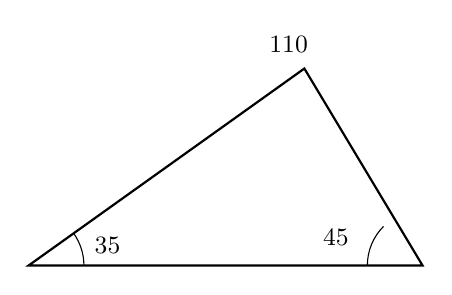
\begin{tikzpicture}[scale=1]
  \draw[thick] (0,0) -- (5,0) -- (3.5,2.5) -- cycle;
  \draw (0.7,0) arc[start angle=0,end angle=35,radius=0.7];
  \node at (1.0,0.25) {\small $35°$};
  \draw (4.3,0) arc[start angle=180,end angle=135,radius=0.7];
  \node at (3.9,0.35) {\small $45°$};
  \node at (3.3,2.8) {\small $110°$};
\end{tikzpicture}
\end{center}
\end{questionText}
\choiceA{Yes, because $35 + 45 + 110 = 190$}
\choiceB{Yes, because all angles are positive}
\choiceC{No, because the angles sum to $190°$ instead of $180°$}
\choiceD{No, because one angle is greater than $90°$}
\correctAnswer{C}
\explanation{$35 + 45 + 110 = 190 \neq 180$. Triangle angles must sum to exactly $180°$, so this triangle is not valid.}
\end{practiceQuestion}

\begin{practiceQuestion}{6-4-q27}{gmc}
\begin{questionText}
The table below shows four sets of triangle conditions. Which one produces a unique triangle?

\begin{center}
\begin{tabular}{|c|l|l|}
\hline
\textbf{Set} & \textbf{Given Information} & \textbf{Condition} \\
\hline
A & Angles: $50°$, $60°$, $70°$ & AAA \\
\hline
B & Sides: $3$, $4$, $5$ & SSS \\
\hline
C & Angles: $45°$, $90°$, $45°$ & AAA \\
\hline
D & One side: $8$ cm & --- \\
\hline
\end{tabular}
\end{center}
\end{questionText}
\choiceA{Set A}
\choiceB{Set B}
\choiceC{Set C}
\choiceD{Set D}
\correctAnswer{B}
\explanation{SSS with valid side lengths ($3 + 4 = 7 > 5$, etc.) produces exactly one unique triangle. AAA gives many triangles, and one side alone is insufficient.}
\end{practiceQuestion}

\begin{practiceQuestion}{6-4-q28}{gmc}
\begin{questionText}
The diagram shows two triangles. Both have angles $30°$, $60°$, and $90°$, but different side lengths. What does this demonstrate?

\begin{center}
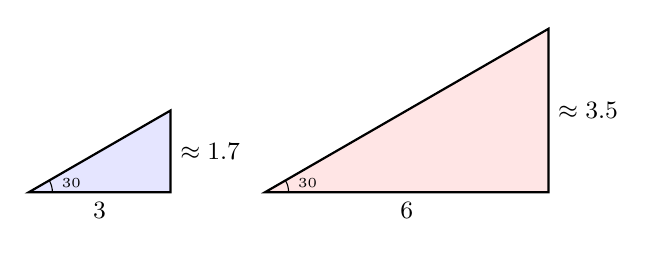
\begin{tikzpicture}[scale=0.6]
  % Small triangle
  \draw[thick,fill=blue!10] (0,0) -- (3,0) -- (3,1.73) -- cycle;
  \node[below] at (1.5,0) {\small $3$};
  \node[right] at (3,0.86) {\small $\approx 1.7$};
  \draw (0.5,0) arc[start angle=0,end angle=30,radius=0.5];
  \node at (0.9,0.2) {\tiny $30°$};
  % Large triangle
  \draw[thick,fill=red!10] (5,0) -- (11,0) -- (11,3.46) -- cycle;
  \node[below] at (8,0) {\small $6$};
  \node[right] at (11,1.73) {\small $\approx 3.5$};
  \draw (5.5,0) arc[start angle=0,end angle=30,radius=0.5];
  \node at (5.9,0.2) {\tiny $30°$};
\end{tikzpicture}
\end{center}
\end{questionText}
\choiceA{SSS produces multiple triangles}
\choiceB{AAA produces a unique triangle}
\choiceC{AAA produces multiple triangles of different sizes}
\choiceD{These two triangles are congruent}
\correctAnswer{C}
\explanation{Both triangles have the same angles but different side lengths. AAA determines shape but not size, so many triangles are possible.}
\end{practiceQuestion}

\begin{practiceQuestion}{6-4-q29}{gsa}
\begin{questionText}
Look at the triangle below. Two sides and the included angle are given. What is the condition type, and is the triangle unique?

\begin{center}
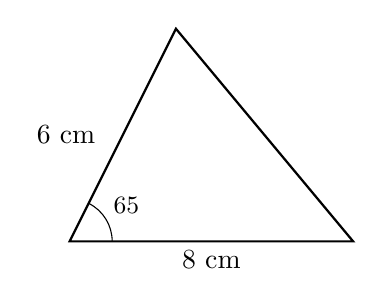
\begin{tikzpicture}[scale=0.9]
  \draw[thick] (0,0) -- (4,0) -- (1.5,3) -- cycle;
  \node[below] at (2,0) {$8$ cm};
  \node[left] at (0.5,1.5) {$6$ cm};
  \draw (0.6,0) arc[start angle=0,end angle=63,radius=0.6];
  \node at (0.8,0.5) {\small $65°$};
\end{tikzpicture}
\end{center}
\end{questionText}
\correctAnswer{SAS; yes, the triangle is unique}
\explanation{Two sides ($8$ cm and $6$ cm) and the included angle ($65°$) give the SAS condition. SAS always produces exactly one unique triangle.}
\end{practiceQuestion}

\begin{practiceQuestion}{6-4-q30}{gsa}
\begin{questionText}
The diagram shows a triangle with the three side lengths labeled. Does it satisfy the triangle inequality? If so, is it unique?

\begin{center}
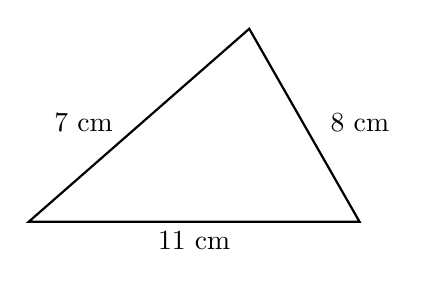
\begin{tikzpicture}[scale=0.7]
  \draw[thick] (0,0) -- (6,0) -- (4,3.5) -- cycle;
  \node[below] at (3,0) {$11$ cm};
  \node[left] at (1.7,1.8) {$7$ cm};
  \node[right] at (5.3,1.8) {$8$ cm};
\end{tikzpicture}
\end{center}
\end{questionText}
\correctAnswer{Yes, it satisfies the inequality and is unique}
\explanation{$7 + 8 = 15 > 11$ \checkmark, $7 + 11 = 18 > 8$ \checkmark, $8 + 11 = 19 > 7$ \checkmark. SSS with valid lengths produces exactly one unique triangle.}
\end{practiceQuestion}
